
\paragraph{} By researching and sifting through a large number of cycling routes, we optimize one route which satisfies almost every requirements\footnote{https://www.strava.com/activities/1178477346/overview}. This course [\ref{route}] is located in Berkeley, USA, passing through Greezly Peak and Berkeley Hills and finanlly ending up back at Berkeley. Riders will complete this course with many sharp curves and nontrivial road grades for a total of 28.26 kilometers with a total elevation gain of 564 meters.
% TODO: \usepackage{graphicx} required
\begin{figure}[h]
	\centering
	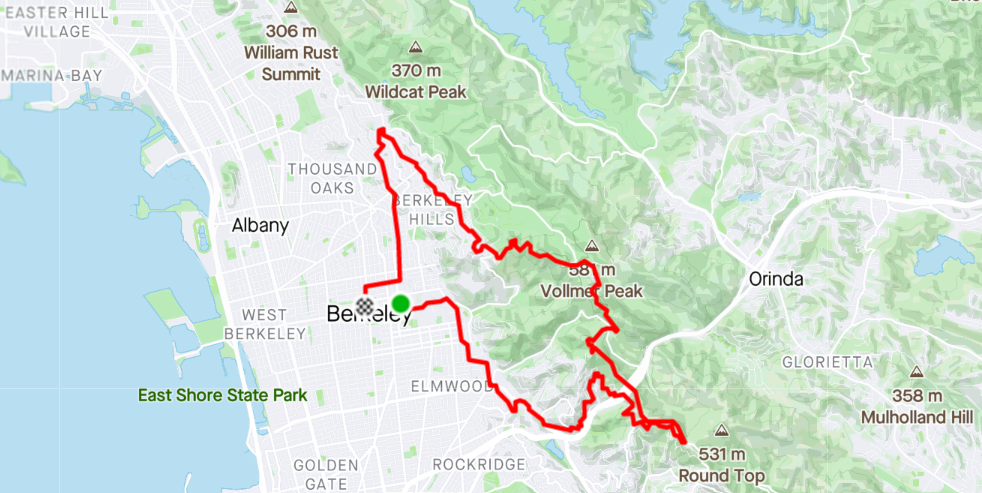
\includegraphics[width=1\linewidth]{image/route}
	\caption{Self-designed route}
	\label{route}
\end{figure}

\par From the circuit profile, after setting off, riders will head on a continuous uphill reaching 4.5 per cent gradient on average[\ref{self1}]. Then, the rolling roads include other climbs which are gentler than the previous course. After reaching the peak, riders will face downhill of almost 10 kilometers along the twists and turns to the finish.
% TODO: \usepackage{graphicx} required
\begin{figure}[h]
	\centering
	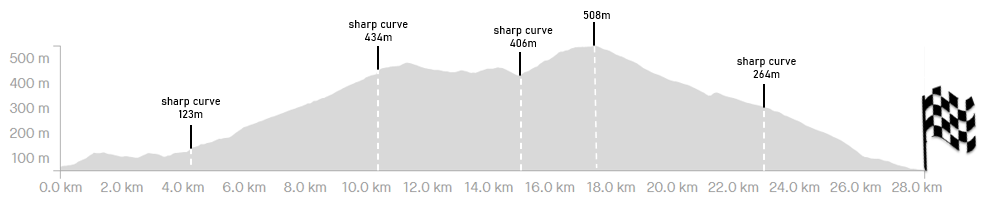
\includegraphics[width=0.9\linewidth]{image/self1}
	\caption{Topographic profile of self-designed course}
	\label{self1}
\end{figure}
\par By applying our model into our self-designed route, the optimal ride planning can be derived [\ref{time3}]. 
\begin{table}[h]
	%	\renewcommand\arraystretch{1.3}
	\setlength{\belowcaptionskip}{0.2cm}
	\setlength\tabcolsep{16pt}%调列距
	\centering
	\caption{ Minimum time to finish self-designed course}
	\begin{tabular}{ccccc}
		\toprule[2pt]
		&$ T_1$(min)    & $T_2$(min)    & $T_3$ (min)   & Total(min) \\
		\midrule
    MTT   & 28:51 & 5:37  & 7:14  & 41:42 \\
FTT   & 32:55 & 5:41  & 8:49  & 47:25 \\
\bottomrule[2pt]
\end{tabular}%
\label{time3}%
\end{table}%
\par Also, an amateur completed the track and uploaded his ride stats on the website. We compare the simulated data to his ride data [\ref{rider3}], and find that the rider lags behind our MTT and FTT riders. It's easy to explain: our riders are world-class athletes, while the strava user is an  amateur. As a result, our model can be correctly applied and proved again. 
% TODO: \usepackage{graphicx} required
\begin{figure}[h]
	\centering
	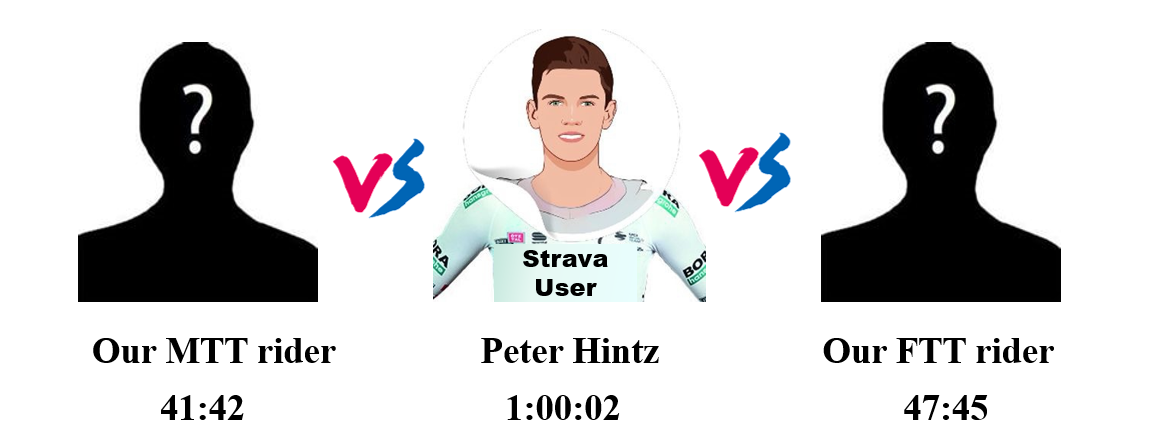
\includegraphics[width=0.7\linewidth]{image/rider3}
	\caption{Our virtual riders and participants of self-designed time trial}
	\label{rider3}
\end{figure}
